% \iffalse meta-comment
%
% Copyright (C) 2011 by Enrico Jörns
% -----------------------------------
%
% This file may be distributed and/or modified under the
% conditions of the LaTeX Project Public License, either version 1.2
% of this license or (at your option) any later version.
% The latest version of this license is in:
%
%   http://www.latex-project.org/lppl.txt
%
% and version 1.2 or later is part of all distributions of LaTeX
% version 1999/12/01 or later.
%
% \fi
%
% \CheckSum{0}
%
% \CharacterTable
%  {Upper-case    \A\B\C\D\E\F\G\H\I\J\K\L\M\N\O\P\Q\R\S\T\U\V\W\X\Y\Z
%   Lower-case    \a\b\c\d\e\f\g\h\i\j\k\l\m\n\o\p\q\r\s\t\u\v\w\x\y\z
%   Digits        \0\1\2\3\4\5\6\7\8\9
%   Exclamation   \!     Double quote  \"     Hash (number) \#
%   Dollar        \$     Percent       \%     Ampersand     \&
%   Acute accent  \'     Left paren    \(     Right paren   \)
%   Asterisk      \*     Plus          \+     Comma         \,
%   Minus         \-     Point         \.     Solidus       \/
%   Colon         \:     Semicolon     \;     Less than     \<
%   Equals        \=     Greater than  \>     Question mark \?
%   Commercial at \@     Left bracket  \[     Backslash     \\
%   Right bracket \]     Circumflex    \^     Underscore    \_
%   Grave accent  \`     Left brace    \{     Vertical bar  \|
%   Right brace   \}     Tilde         \~}
%
% \iffalse
%
%<*driver>
\documentclass{ltxdoc}
\usepackage[ngerman]{babel}
\usepackage[utf8]{inputenc}
\usepackage{nexus}
\usepackage[colorlinks, linkcolor=blue]{hyperref}
\usepackage{tabularx}
\EnableCrossrefs
\CodelineIndex
\RecordChanges
\begin{document}
  \DocInput{beamerinnerthemetubs.dtx}
\end{document}
%</driver>
% \fi
%
% \newenvironment{key}[2]{\expandafter\macro\expandafter{`#2'}}{\endmacro}
% \newenvironment{Options}%
%  {\begin{list}{}{%
%   \renewcommand{\makelabel}[1]{\texttt{##1}\hfil}%
%   \setlength{\itemsep}{-.5\parsep}
%   \settowidth{\labelwidth}{\texttt{xxxxxxxxxxx\space}}%
%   \setlength{\leftmargin}{\labelwidth}%
%   \addtolength{\leftmargin}{\labelsep}}%
%   \raggedright}
%  {\end{list}}
%
% \changes{v1.0}{ 2011 / 08 / 23 }{Initial version}
%
% \GetFileInfo{beamerinnerthemetubs.sty}
%
% \DoNotIndex{ list of control sequences }
%
% \title{\textsf{beamerinnerthemetubs} -- 
%   beamer-Farbschema für \emph{tubslatex}\thanks{This document
%   corresponds to \textsf{beamerinnerthemetubs}~\fileversion,
%   dated \filedate.}}
% \author{Enrico Jörns \\ \texttt{e dot joerns at tu minus bs dot de}}
%
% \maketitle
%
% \begin{abstract}
%   Diese Datei stellt das Farbschema für latex-beamer-Präsentationen im
%   Corporate Design dar.
% \end{abstract}
%
% \StopEventually{\PrintIndex}
%
% \section{Implementierung}
%
%
%    \begin{macrocode}
%<*innertheme>
\ProvidesPackage{beamerinnerthemetubs}[2011/09/10 v1.0 Beamer-Inner-Template TuBs]
%    \end{macrocode}
%
% Lade Pakete.
%    \begin{macrocode}
\RequirePackage{ifthen}
\RequirePackage{relsize}[1999/11/01]
\RequirePackage{printlen}
\RequirePackage{tubsbeamersizes}
\RequirePackage{tubslogo}
%    \end{macrocode}
%
%
% \subsection{Optionen}
%
%
%    \begin{key}{}{shadow}
%    \begin{macrocode}
\DeclareOptionBeamer{shadow}[true]{\def\beamer@themerounded@shadow{#1}}
%    \end{macrocode}
%    \end{key}
%
% Optionen behandel
%    \begin{macrocode}
\ExecuteOptionsBeamer{shadow=false}
\ProcessOptionsBeamer\relax
%    \end{macrocode}
%
%
% \subsection{Titelgrafik und Logo}
%
%
%    \begin{macro}{\tuDefaultTitlegraphic}
% Lädt Standard-Titelgraphik
%    \begin{macrocode}
\newcommand{\tuDefaultTitlegraphic}{%
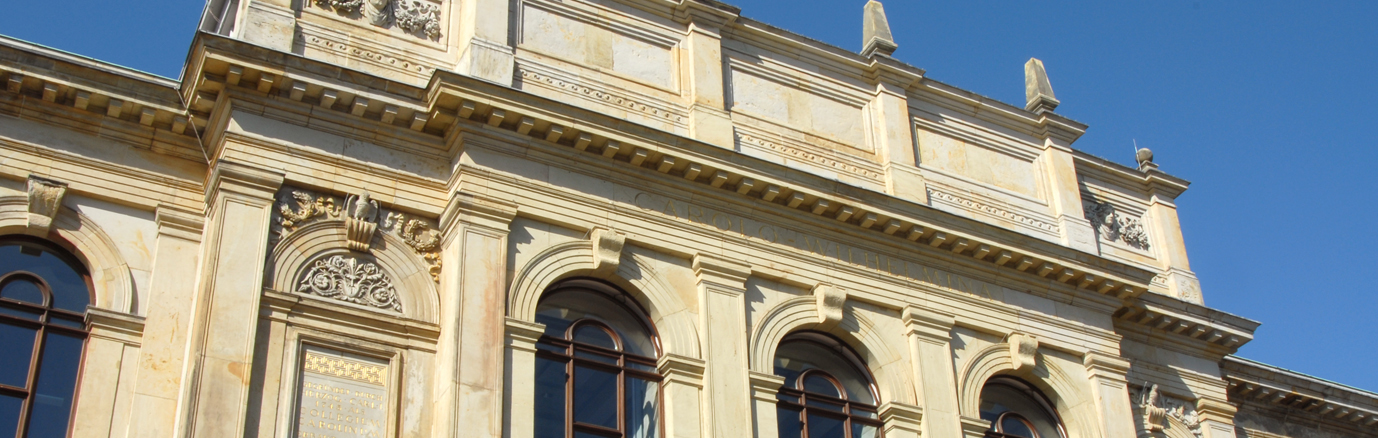
\includegraphics[width=\titlegraphicswidth]{defaulttitlepicture}}
%    \end{macrocode}
%    \end{macro}
%
%
%    \begin{macrocode}
%NOTE: beamer redefines includegraphics and drops the starred version... :/
\newcommand\tubs@imagefit{cropped}
\newcommand\@img@scale@param{}%
%    \end{macrocode}
%
%    \begin{macro}{\tubs@calc@autoscale}
%    \begin{macrocode}
\newcommand\tubs@calc@autoscale[1]{%
  \newdimen\@image@xorig%
  \newdimen\@image@xcalc%
  \newdimen\@image@yorig%
  \newdimen\@image@ycalc%
  \ifthenelse{\equal{\tubs@imagefit}{scaled}}{%
    \renewcommand\@img@scale@param{clip,%
        height=\titlegraphicsheight,
        width=\titlegraphicswidth}
  }{\ifthenelse{\equal{\tubs@imagefit}{cropped}}{%
      % Ermittelt, ob das Bild an den Seiten oder oben und unten beschnitten
      % werden muss, um in den Darstellungsbereich zu passen
      % Dazu wird die Höhe des auf korrekte Breite skalierten Bildes
      % mit der Höhe des Darstellungsbereichs verglichen und entsprechend
      % eine crop-Option gesetzt.
      \settoheight{\@image@ycalc}{%
        \includegraphics[clip,width=\titlegraphicswidth]{#1}}
      \ifthenelse{\lengthtest{\@image@ycalc>\titlegraphicsheight}}{%
        \renewcommand{\tubs@imagefit}{cropy}
      }{%
        \renewcommand{\tubs@imagefit}{cropx}
      }
    }{}
    \ifthenelse{\equal{\tubs@imagefit}{cropy}}{%
      % Berechne abzuschneidende Ränder (oben+unten)
      % Dazu wird die Differenz zwischen Darstellungsbereich und Höhe des
      % korrekt auf die Breite skalierten Bildes berechnet und mit dem
      % ermittelten Skalierungsfaktor multipliziert, sowie durch 2 geteilt.
      % Das Ergebnis wir dann einmal am oberen und einmal am unteren Teil
      % des (Original-)Bildes mit Hilfe der 'trim'-Option abgeschnitten.
      \settoheight{\@image@yorig}{%
        \includegraphics[clip]{#1}}%
      \settoheight{\@image@ycalc}{%
        \includegraphics[clip,width=\titlegraphicswidth]{#1}}%
      \setlength{\@image@ycalc}{(\@image@ycalc-\titlegraphicsheight)*\ratio{\@image@yorig}{\@image@ycalc}}
      \setlength{\@image@ycalc}{0.5\@image@ycalc}%
      \renewcommand\@img@scale@param{clip,%
          width=\titlegraphicswidth,
          trim=0pt {\@image@ycalc} 0pt {\@image@ycalc}}%
    }{\ifthenelse{\equal{\tubs@imagefit}{cropx}}{%
      \settowidth{\@image@xorig}{%
        \includegraphics[clip]{#1}}%
      \settowidth{\@image@xcalc}{%
        \includegraphics[clip,height=\titlegraphicsheight]{#1}}%
      \setlength{\@image@xcalc}{(\@image@xcalc-(\titlegraphicswidth))*\ratio{\@image@xorig}{\@image@xcalc}}
      \setlength{\@image@xcalc}{0.5\@image@xcalc}%
      \renewcommand\@img@scale@param{clip,%
          height=\titlegraphicsheight,
          trim={\@image@xcalc} 0pt {\@image@xcalc} 0pt}%
    }{\ifthenelse{\equal{\tubs@imagefit}{keepsize}}{%
      \renewcommand\@img@scale@param{}%
    }{}}}%
  }%
}
%    \end{macrocode}
%    \end{macro}
%
% \paragraph{Imagefit-Keys}
%
%    \begin{key}{}{scaled}
% Horizontal + vertikal Skalieren
%    \begin{macrocode}
\define@key{tubs@titlegraphic}{scaled}[true]{
  \renewcommand\tubs@imagefit{scaled}
}
%    \end{macrocode}
%    \end{key}
%
%    \begin{key}{}{cropx}
% Skalieren auf Höhe, Zuschneiden auf Breite
%    \begin{macrocode}
\define@key{tubs@titlegraphic}{clipx}[true]{
  \renewcommand\tubs@imagefit{cropx}
}
\define@key{tubs@titlegraphic}{cropx}[true]{
  \renewcommand\tubs@imagefit{cropx}
}
%    \end{macrocode}
%    \end{key}
%
%    \begin{key}{}{cropy}
% Skalieren auf Breite, Zuschneiden auf Höhe
%    \begin{macrocode}
\define@key{tubs@titlegraphic}{clipy}[true]{
  \renewcommand\tubs@imagefit{cropy}
}
\define@key{tubs@titlegraphic}{cropy}[true]{
  \renewcommand\tubs@imagefit{cropy}
}
%    \end{macrocode}
%    \end{key}
%
%    \begin{key}{}{cropped}
% Automatisches Skalieren und Zuschneiden
%    \begin{macrocode}
\define@key{tubs@titlegraphic}{clipped}[true]{
  \renewcommand\tubs@imagefit{cropped}
}
\define@key{tubs@titlegraphic}{cropped}[true]{
  \renewcommand\tubs@imagefit{cropped}
}
%    \end{macrocode}
%    \end{key}
%
%    \begin{key}{}{keepsize}
%    \begin{macrocode}
\define@key{tubs@titlegraphic}{keepsize}[true]{
  \renewcommand\tubs@imagefit{keepsize}
}
%    \end{macrocode}
%    \end{key}
%
%
%    \begin{macrocode}
\let\@orig@titlegpraphic\titlegraphic
\newsavebox{\@test@box}
%    \end{macrocode}
%
%    \begin{macro}{\titlegpraphic}
%    \begin{macrocode}
\renewcommand{\titlegraphic}[2][]{%
  \@orig@titlegpraphic{
    \setkeys{tubs@titlegraphic}{cropped,#1}%
    % redefine includegraphics to store information
    \newif\if@incgraphused\@incgraphusedfalse%
    \let\@orig@includegraphics\includegraphics%
    \renewcommand{\includegraphics}[2][\relax]{%
      \@incgraphusedtrue%
      \def\@incgraph@optparam{####1}%
      \def\@incgraph@param{####2}%
      \ifthenelse{\equal{\@incgraph@optparam}{\relax}}{%
        \let\@manipulated@includegraphics\includegraphics
        \let\includegraphics\@orig@includegraphics
        \tubs@calc@autoscale{\@incgraph@param}%
        \let\includegraphics\@manipulated@includegraphics
        \expandafter\@orig@includegraphics\expandafter[\@img@scale@param]{%
                \@incgraph@param}%
      }{%
        \expandafter\@orig@includegraphics\expandafter[\@incgraph@optparam]{%
                \@incgraph@param}%
      }
  }%
  #2}
}
%    \end{macrocode}
%    \end{macro}
%
%
%    \begin{macro}{\logo}
%    \begin{macrocode}
% Höhe des Logos wird automatisch skaliert bei Verwendung von includegraphics
\renewcommand{\logo}[1]{%
  \setbeamertemplate{logo}{%
    \begingroup%
    \presetkeys{Gin}{height=\logoheight,width=0.5\textwidth,keepaspectratio}{}%
    #1%
    \endgroup%
  }%
}
%    \end{macrocode}
%    \end{macro}
%
%
% \subsection{Templates}
%
%    \begin{macrocode}
\mode<presentation>% TODO: Hier ???
%    \end{macrocode}
%
%    \begin{macrocode}
\setbeamertemplate{blocks}[rounded][shadow=\beamer@themerounded@shadow]
%    \end{macrocode}
%
%    \begin{macro}{title page}
%    \begin{macrocode}
%% Trick: To re-define a template from scratch, give it a new name as
%% second argument.
\defbeamertemplate*{title page}{tubs}[1][]{%
  \vspace*{-5.5pt} % korrigierte Nulllinie
  \vspace*{\beamer@CDsenderheight}
  \begin{beamercolorbox}[
      wd=\beamer@CDcommunicationwidth,
      ht=11\beamer@CDgaussunit]
      {titlebarthird}
    \usebeamerfont{title}\centering\inserttitlegraphic%
  \end{beamercolorbox}%
  \vskip-1pt

  \begin{beamercolorbox}[wd=\beamer@CDcommunicationwidth,
      ht=9\beamer@CDgaussunit]
      {titlebarsecond}
    \hspace*{\beamer@leftmarginwidth}
    \parbox[b][9\beamer@CDgaussunit][c]{\beamer@titlepagetextwidth}{%
    \vskip1.0ex\par
    \usebeamerfont{title}\inserttitle \par%
    \vskip0.8ex\par
    \usebeamerfont{subtitle}\insertsubtitle \par%
    \vskip1.6ex\par
    \usebeamerfont{author}\insertauthor, \insertdate}
  \end{beamercolorbox}%
  \vskip-1pt

  {\tiny
  \begin{beamercolorbox}[wd=\beamer@CDcommunicationwidth,
      ht=\beamer@CDgaussunit]
      {titlebarlow}
  \end{beamercolorbox}}%
  \vspace*{-24.1\beamer@CDgaussunit}

  \begin{beamercolorbox}[wd=\beamer@CDcommunicationwidth,
      ht=4\beamer@CDgaussunit]
      {structure}
    \hspace*{-\beamer@CDborderwidth}\tubslogoAbs{37mm}
  \end{beamercolorbox}
  \vspace*{-20mm}

  \begin{beamercolorbox}[
      wd=\beamer@CDcommunicationwidth,ht=4\beamer@CDgaussunit]
      {structure}
    \vbox to 4\beamer@CDgaussunit{%
    \vfill
    \parbox{\beamer@CDcommunicationwidth}{%
      \usebeamerfont{author}\raggedleft\insertlogo}
    \vfill}
  \end{beamercolorbox}
  \vspace*{22\beamer@CDgaussunit}
}
%    \end{macrocode}
%    \end{macro}
%
%    \begin{macro}{part page}
%    \begin{macrocode}
\defbeamertemplate*{part page}{tubs}[1][]{%
  \begin{centering}
    {\usebeamerfont{part name}\usebeamercolor[fg]{part name}\partname~\insertromanpartnumber}
    \vskip1em\par
    \begin{beamercolorbox}[sep=8pt,center,#1]{part title}
      \usebeamerfont{part title}\insertpart\par
    \end{beamercolorbox}
  \end{centering}
}
%    \end{macrocode}
%    \end{macro}
%
%    \begin{macro}{narrowitemize}
% Itemize environment with narrower lines
%    \begin{macrocode}
\newenvironment{narrowitemize}{%
  \begin{itemize}%
    \setlength{\itemsep}{0pt}%
}{%
  \end{itemize}%
}
%    \end{macrocode}
%    \end{macro}
%
%    \begin{macro}{emptyitemize}
% Itemize environment with narrower lines and with no item signs
%    \begin{macrocode}
\newenvironment{emptyitemize}{%
  \setbeamertemplate{itemize item}{\ }
  \setbeamertemplate{itemize subitem}{\rule[0.17em]{0.25em}{0.25em}}
  \begin{itemize}%
    \setlength{\itemsep}{0pt}%
}{%
  \end{itemize}%
}
%    \end{macrocode}
%    \end{macro}
%
%    \begin{macrocode}
%  Squares for items
\defbeamertemplate*{itemize item}{tubs}{\rule[0.15em]{0.3em}{0.3em}}
\defbeamertemplate*{itemize subitem}{tubs}{\rule[0.17em]{0.25em}{0.25em}}
%  dash for subsubitems
\defbeamertemplate*{itemize subsubitem}{tubs}{\textbf{\textendash}}
\defbeamertemplate*{itemize subsubsubitem}{tubs}{\textperiodcentered}
%    \end{macrocode}
%
%    \begin{macrocode}
\defbeamertemplate{section in toc}{tubs}{%
  \leavevmode\normalsize\raise-1.5pt\hbox{\rule[0.15em]{0.3em}{0.3em}}\kern1.25ex
  \inserttocsection\par
}
%    \end{macrocode}
%
%    \begin{macrocode}
\defbeamertemplate{subsection in toc}{tubs}{%
  \leavevmode\leftskip=1.5em\hbox{\rule[0.17em]{0.25em}{0.25em}}%
  \kern1ex\inserttocsubsection\par
}
%    \end{macrocode}
%
%    \begin{macrocode}
\defbeamertemplate{subsubsection in toc}{tubs}{%
  \leavevmode\normalsize\usebeamerfont{subsection in
    toc}\leftskip=3em\usebeamerfont{subsubsection in toc}%
  \hbox{\textasteriskcentered}%
  \kern0.75ex\inserttocsubsubsection\par
}
%    \end{macrocode}
%
%    \begin{macrocode}
\setbeamertemplate{items}[tubs]
\setbeamertemplate{sections/subsections in toc}[tubs]
%    \end{macrocode}
%
%    \begin{macrocode}
\setlength{\leftmargini}{1.3em}
\setlength{\leftmarginii}{1.3em}
\setlength{\leftmarginiii}{1.3em}
\setlength{\leftmarginiv}{1.3em}
%    \end{macrocode}
%
%    \begin{macrocode}
\setbeamercovered{transparent}
%    \end{macrocode}
%
%    \begin{macrocode}
\mode<all>
%</innertheme>
%    \end{macrocode}
%
% \Finale
\endinput
%

